\chapter{Tecnologia - Recurso essencial para a competitividade da empresa industrial}
\label{chap:tecnologia_recurso}

Tecnologia é o estudo sistemático sobre técnicas, processos, métodos e instrumentos de domínio da atividades humana. No setor industrial, este ofício representa o controle destas técnicas e também a capacidade de implementação de novas funcionalidades em máquinas para que estas possam operar de forma autônoma e sem o conhecimento do seu funcionamento interno. Em resumo, a tecnologia pode ser descrita como a arte de desenvolver e utilizar novas ferramentas.

É definida como Tecnologia do Produto aquela introduzida no produto e usada na criação do seu projeto ou no decorrer do seu desenvolvimento. De acordo com o Manual de Apoio ao Preenchimento da Pintec (2014) %!tem que citar aqui
, a inovação de produto consiste em criar modificações nos atributos dos bens ou serviços, tais como mudanças operacionais e na forma como ele é percebido pelos consumidores.

A tecnologia empregada na rotina de produção de um produto, destinada a fazer com que sejam atingidas as metas estabelecidas pela empresa é chamada Tecnologia de Processo. O tipo de produto a ser produzido é quem dita a tecnologia usada no processo industrial, ao lado da quantidade e volume que serão fabricados.

É exemplo de tecnologia de processos a empregada na produção de materiais. O uso de robôs e outras máquinas vem crescendo e se consolidando como algo indispensável. O uso de máquinas de corte, furadeiras e \ac{CNC} complementam a tendencia no uso da automação.

O processamento de informações, assim como a \ac{TI}, vem avançando e se popularizando exponencialmente. Tem a intenção de ser abrangente e atua como técnologia principal ou auxiliar em quase todos os ramos de trabalho.

O emprego das tecnologias permitem a constante inovação de produtos e processos e garantem a presença competitiva no mercado. Produtos novos, modificados e mais eficientes aumentam a procura e melhoram a opinião do cliente a respeito da empresa.


\section{Aplicação Prática}
\label{sec:tecnologia_recurso_aplicacao}

Como o produto da SunBurn é a energia elétrica gerada a partir da energia solar, o produto em si já está estabelecido de uma forma geral, não havendo possibilidade de inovação na sua forma primária. As inovações podem então ocorrer no seu processo produtivo com aumento da eficiência de conversão, melhoria na qualidade do produto entregue e adequação do produto, níveis de tensão, aos requisitos do cliente.

O processo produtivo básico, tal como indicado no Capítulo \ref{chap:tipos_de_processo_de_producao}, é constituído principalmente de painéis solares fotovoltáicos, inversores de tensão, transformadores e circuito de proteção. Em linhas gerais, as maiores inovações tecnológicas atuais ocorrem sobre os painéis fotovoltáicos e inversores, com foco principal no aumento da eficiência da conversão de energia. A SunBurn apresenta atualmente um plano de implantação de produção de painéis fotovoltáicos em território nacional.

Em relação à manutenção do parque industrial, a SunBurn utiliza um robô tele-operado para executar a limpeza do entorno dos painéis solares \cite{energreen}. A configuração padrão deste robô está disposto na Figura \ref{fig:energreen}.

\begin{figure}
  \caption{RoboGREEN evo.}
  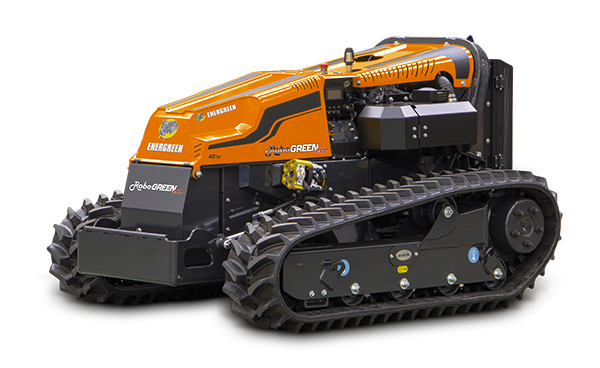
\includegraphics[width=1\textwidth]{images/robogreen_evo.png}
  \legend{Fonte: \cite{energreen}.}
  \label{fig:energreen}
\end{figure}
